\begin{dang}{Tìm Max-min qua bảng biến thiên, đồ thị}
    Để tìm max min của hàm số $y=f(x)$ trên miền $\mathscr{D}$, ta thường lập bảng biến thiên của hàm số $y=f(x)$ trên $\mathscr{D}$. Từ bảng biến thiên, ta kết luận:
    \begin{multicols}{2}
        \begin{itemize}
            \item  Điểm ở vị trí cao nhất $\longrightarrow$ Kết luận max;
            \item  Điểm ở vị trí thấp nhất $\longrightarrow$ Kết luận min.
        \end{itemize}
    \end{multicols}
\end{dang}
\begin{vd}%[Dự án tex hóa đề cương Mariecurie - Biên soạn Thầy Nguyễn Ngọc Nguyên]
    \immini{ Cho hàm số $y=f(x)$ có bảng biến thiên như hình vẽ, tìm Max-min của $y=f(x)$ trên
        \begin{listEX}[2]
            \item $(-\infty; -4]$.
            \item $(-\infty; 1)$.
            \item $(-\infty; 6)$.
            \item $(1; +\infty)$.
            \item $[6; +\infty)$.
            \item $(-4;1)$.
        \end{listEX}
    }{
\begin{tikzpicture}
            \tkzTabInit[espcl=2,lgt=1]
            {$x$ /.7, $y'$ /.7,$y$ /2.3}
            {$-\infty$, $-4$, $1$, $6$, $+\infty$}
            \tkzTabLine{,+,$0$, -, d, +, d ,-,}
            \tkzTabVar{ -/$-\infty$,+/$5$,-D+/$-\infty$/$+\infty$,-/$-7$, +/$2$}
    \end{tikzpicture}}
    \loigiai{}
\end{vd}
\begin{vd}
    \immini{Cho hàm số $y=f(x)$ có đồ thị như hình vẽ. Tìm Max-min của
        \begin{listEX}[2]
            \item $y=f(x)$ trên $[-2;3]$.
            \item $y=f(x)$ trên $[0;3]$.
            \item $y=|f(x)|$.
            \item $y=f(|x|)$.
            \item $y=f(2\sin3x+1)$.
            \item $y=f(3\cos^25x-2)$.
        \end{listEX}
    }{
        \begin{tikzpicture}[>=stealth, font=\scriptsize, line join=round, line cap=round,y=.8cm]
            \begin{scope}[scale=.8]
                \def\a{-1} \def\b{0} \def\c{2} % Hệ số
                \def\xmin{-2.5} \def\xmax{3.7}
                \def\ymin{-2.5} \def\ymax{4}
                %	\draw[color=gray!50,dashed] (\xmin,\ymin) grid (\xmax,\ymax);
                \draw[->] (\xmin,0)--(\xmax,0) node [below]{$x$};
                \draw[->] (0,\ymin)--(0,\ymax) node [left]{$y$};
                \draw (1,1)--(3,3);
                \draw[dashed] (1,0)--(1,1)--(0,1);
                \draw[dashed] (3,0)--(3,3)--(0,3);
                \draw[dashed] (-2,0)--(-2,-2)--(0,-2);
                \node at (0,0) [below right]{$O$};
                \clip (\xmin+0.1,\ymin+0.1) rectangle (\xmax-0.5,\ymax-0.1);
                \draw[smooth,samples=300][domain=-2:1] plot(\x,{\a*(\x)^2+\b*(\x)+\c});
                \foreach \x in {-2,-1,1,2,3}
                \draw[thin] (\x,1pt)--(\x,-1pt) node [below] {$\x$};
                \foreach \y in {-2,1,2,3}
                \draw[thin] (1pt,\y)--(-1pt,\y) node [above left] {$\y$};
            \end{scope}
    \end{tikzpicture}}
    \loigiai{}
\end{vd}
\begin{vd}
    \immini{Cho hàm số $y=f(x)$ có đồ thị hàm số $y=f'(x)$ như hình vẽ. Tìm Max-min của hàm số
        \begin{listEX}
            \item[a)] $y=f(x)$ trên $[-2;2]$, biết $f(2)<f(-2)$.
            \item[b)] $y=f(x)$ trên $[-2;2]$, biết $f(1)+f(2)=f(-1)+f(-2)$.
            \item[c)] $y=f^3(x)+3f(x)$ trên $[-2;2]$, biết $f(2)+f(0)-2f(-1)=f(-2)-f(1)$.
        \end{listEX}
    }{
        \begin{tikzpicture}[>=stealth,x=1cm,y=.7cm,scale=0.9,font=\footnotesize]
            \path
            (2,0) coordinate (B2)
            (-1.7,1.7) coordinate (N)
            (-0.7,-0.7) coordinate (P)
            (0,0) coordinate (O)node[above right]{$ O$}
            (1.7,-1.7) coordinate (Q)
            ($(B2)!(N)!(O)$) coordinate (A1)node[below]{$ -2 $}
            ($(B2)!(Q)!(O)$) coordinate (B1)node[above]{$ 2 $}
            ;
            %	\draw[red] (N)--(P)--(O)--(Q);
            \draw[name path=ox] (O)--(-2,0);
            \draw[name path=fx]
            (N)..controls +(-70:1) and+(170:0.25)..
            (P)..controls +(9:0.25) and+(-170:0.25)..(O)
            ..controls +(-5:0.35) and+(140:0.25)..(Q)
            ;
            \draw[dashed](N)--(A1) (Q)--(B1);
            \path[name intersections={of=fx and ox, by={A3,A2}}] ;
            %Vẽ hệ trục tọa dộ:
            \draw[->] (-2,0)--(0,0)--(2,0) node[below]{$x$};
            \draw[->] (0,-2) --(0,2.2) node[left]{$y$};
            %	Node các điểm
            \foreach \p in {N,O,Q}
            \fill (\p) circle (1.5pt) ;
            \fill(A3) circle (1.5pt) node[above right]{$ -1 $};
    \end{tikzpicture}}
    \loigiai{}
\end{vd}
\BTTN
\Opensolutionfile{ans}[ans/2D1-3-DANG-1]
\begin{ex}%[2D1B3-1]
    \immini{Cho hàm số $f(x)$ liên tục trên đoạn $[-1;3]$ và có đồ thị như hình vẽ. Gọi $M$ và $m$ lần lượt là giá trị lớn nhất, giá trị nhỏ nhất của hàm số đã cho trên $[-1;3]$. Giá trị $M-m$ bằng
        \choice[2]
        {$0$}
        {\True $5$}
        {$4$}
        {$1$}}{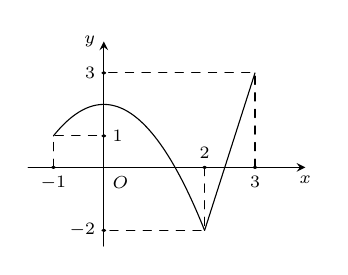
\begin{tikzpicture}[scale=0.8,xscale=0.8,yscale=0.5,>=stealth, font=\scriptsize, line join=round, line cap=round]
            \def\a{-1} \def\b{0} \def\c{2} % Hệ số
            \def\xmin{-1.5} \def\xmax{4}
            \def\ymin{-2.5} \def\ymax{4}
            %	\draw[color=gray!50,dashed] (\xmin,\ymin) grid (\xmax,\ymax);
            \draw[->] (\xmin,0)--(\xmax,0) node [below]{$x$};
            \draw[->] (0,\ymin)--(0,\ymax) node [left]{$y$};
            \node at (0,0) [below right]{$O$};
            \clip (\xmin+0.1,\ymin+0.1) rectangle (\xmax-0.5,\ymax-0.1);
            \draw[smooth,samples=300,domain=-1:2] plot(\x,{\a*(\x)^2+\b*(\x)+\c});
            \draw(2,-2)--(3,3);
            \draw[fill=black](-1,0)node[below]{$-1$}circle(1pt)
            (0,1)node[right]{$1$}circle(1pt)
            (2,0)node[above]{$2$}circle(1pt)
            (0,-2)node[left]{$-2$}circle(1pt)
            (3,0)node[below]{$3$}circle(1pt)
            (0,3)node[left]{$3$}circle(1pt)
            ;
            \draw[dashed](3,0)|-(0,3);
            \draw[dashed](-1,0)|-(0,1);
            \draw[dashed](2,0)|-(0,-2);
    \end{tikzpicture}}
    \loigiai{
        Dựa vào đồ thị ta có $M=\max\limits_{[-1;3]} f(x)=3$ và $m=\min\limits_{[-1;3]} f(x)=-2$.\\Suy ra $M-m=5$.
    }
\end{ex}
\begin{ex}%[Dự án tex hóa đề cương Mariecurie - Biên soạn Thầy Nguyễn Ngọc Nguyên]%[2D1B3-1]
    \immini{Cho hàm số $f(x)$ liên tục trên đoạn $[-2;3]$ và có đồ thị như hình bên. Gọi $M,m$ lần lượt là giá trị lớn nhất, nhỏ nhất của hàm số đã cho trên đoạn $[-2;3
        ]$. Giá trị của $M-m$ bằng
        \choice[2]
        {$4$}
        {$1$}
        {\True $3$}
        {$2$}}
    {
        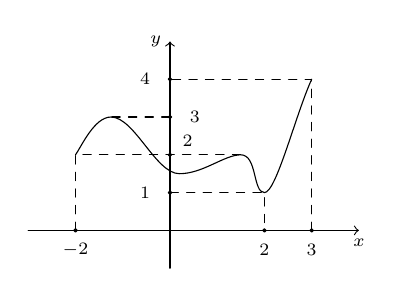
\begin{tikzpicture}[line cap=round, line join=round,font=\scriptsize,y=.8cm]
            \begin{scope}[scale=.6]
                \draw[->](-3,0)--(4,0)node[below]{$x$};
                \draw[->](0,-1)--(0,5)node[left]{$y$};
                \draw(-2,2)..controls ++(60:0.25) and ++(180:0.35)..(-1.25,3)..controls++(0:.5) and ++(180:0.5)..(0.2,1.5)..controls++(0:0.5) and ++(180:0.35)..(1.5,2)..controls++(0:0.35) and ++(180:0.25)..(2,1)..controls++(0:0.25) and++(-110:1)..(3,4);
                \draw[dashed](-2,0)--(-2,2)--(1.5,2)(0,1)--(2,1)--(2,0)(3,0)--(3,4)--(0,4)(0,3)--(-1.25,3);
                \foreach \x/\y/\m/\g in{-2/0/-2/-90,0/2/2/45,0/1/1/180,2/0/2/-90,3/0/3/-90,0/3/3/0,0/4/4/180}
                \draw[fill=black](\x,\y)circle(1pt)node[shift={(\g:0.35)}]{$\m$};
            \end{scope}
        \end{tikzpicture}
    }
    \loigiai
    {
        Ta có $M=4$ và $m=1$, do đó $M-m=3$.
    }
\end{ex}
\begin{ex}%[Võ Thị Thùy Trang - DA1]%[2D1Y3-1]
    \immini{Cho hàm số $y=f(x)$ xác định và liên tục trên $[-2;3]$ có bảng biến thiên như hình bên. Gọi $M$, $m$ lần lượt là giá trị lớn nhất và nhỏ nhất của hàm số trên đoạn $\left[-2;3\right]$. Tổng $M+m$ bằng
        \choice
        {$-1$}
        {$3$}
        {\True $1$}
        {$4$}
    }
    {
\begin{tikzpicture}[scale=.76,>=stealth, font=\footnotesize, line join=round, line cap=round]
            \tkzTabInit[nocadre=false,lgt=1.2,espcl=2.5,deltacl=0.6]
            {$x$ /0.6, $y'$ /0.6, $y$ /2.5}
            {$-2$,$0$,$1$,$3$}
            \tkzTabLine{,+,$0$,-,d,+,}
            \tkzTabVar{-/$-2$,+/$2$,-/$1$,+/$3$}
    \end{tikzpicture}}
    \loigiai{
        Ta có $M=\max\limits_{[-2;3]} f(x)=f(3)=3$; $M=\min\limits_{[-2;3]} f(x)=f(-2)=-2$.\\
        nên $M+m=3-2=1$.
    }
\end{ex}
\begin{ex}%[Võ Thị Thùy Trang - DA1]%[2D1Y3-1]
    \immini{Cho hàm số $y=f(x)$ liên tục trên $\mathbb{R}$ và có bảng biến thiên trên đoạn $[-1;4]$ như hình bên dưới. Gọi $M$ và $m$ lần lượt là giá trị lớn nhất và nhỏ nhất của hàm số đã cho trên đoạn $\left[-1;4\right]$. Giá trị của $M+m$ bằng
        \choice
        {$-4$}
        {\True $-28$}
        {$20$}
        {$-20$}
    }
    {
\begin{tikzpicture}[scale=.76,>=stealth, font=\footnotesize, line join=round, line cap=round]
            \tkzTabInit[nocadre=false,lgt=1.2,espcl=2.5,deltacl=0.6]
            {$x$ /0.6, $y'$ /0.6, $y$ /2.5}
            {$-1$,$1$,$3$,$4$}
            \tkzTabLine{,+,$0$,-,$0$,+,}
            \tkzTabVar{-/$-24$,+/$-4$,-/$-8$,+/$-4$}
    \end{tikzpicture}}
    \loigiai{
        Ta có $M=\max\limits_{[-1;4]} f(x)=f(1)=f(4)=-4$; $m=\min\limits_{[-1;4]} f(x)=f(-1)=-24$.\\
        nên $M+m=-4-24=-28$.
    }
\end{ex}
\begin{ex}%[Võ Thị Thùy Trang - DA1]%[2D1B3-2]%5
    \immini{Cho hàm số $y=f(x)$ xác định, liên tục trên đoạn $[-2;2]$ và có đồ thị là đường cong trong hình vẽ bên dưới. Gọi $M$ và $m$ lần lượt là giá trị lớn nhất và nhỏ nhất của hàm số đã cho trên đoạn $[-2;2]$. Giá trị của $M-m$ bằng
        \choice
        {$0$}
        {\True $8$}
        {$4$}
        {$2$}
    }
    {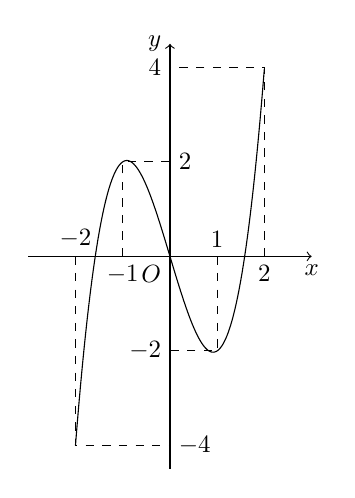
\begin{tikzpicture}[scale=0.6]
            \def\a{4/3} \def\b{0} \def\c{-10/3} \def\d{0} % Hệ số
            \def\xmin{-3} \def\xmax{3}
            \def\ymin{-4.5} \def\ymax{4.5}
            %	\draw[color=gray!50,dashed] (\xmin,\ymin) grid (\xmax,\ymax);
            \draw[->] (\xmin,0)--(\xmax,0) node [below]{$x$};
            \draw[->] (0,\ymin)--(0,\ymax) node [left]{$y$};
            \node at (0,0) [below left]{$O$};
            \draw[dashed] (-2,0) node [above] {$-2$}--(-2,-4)--(0,-4) node [right] {$-4$};
            \draw[dashed] (-1,0) node [below] {$-1$}--(-1,2)--(0,2) node [right] {$2$};
            \draw[dashed] (1,0) node [above] {$1$}--(1,-2)--(0,-2) node [left] {$-2$};
            \draw[dashed] (2,0) node [below] {$2$}--(2,4)--(0,4) node [left] {$4$};
            \clip (\xmin+0.1,\ymin+0.1) rectangle (\xmax-0.5,\ymax-0.1);
            \draw[smooth,samples=300][domain=-2:2] plot(\x,{\a*(\x)^3+\b*(\x)^2+\c*(\x)+\d});
    \end{tikzpicture}}
    \loigiai{
        Ta có $M=\max\limits_{[-2;2]} f(x)=f(2)=4$; $m=\min\limits_{[-2;2]} f(x)=f(-2)=-4$.\\
        nên $M-m=4-(-4)=8$.
    }
\end{ex}
\begin{ex}%[Võ Thị Thùy Trang - DA1]%[2D1B3-2]%6
    \immini{Cho hàm số $y=f(x)$ xác định và liên tục trên $\mathbb{R}$ có đồ thị bên dưới. Gọi $M$ và $m$ lần lượt là giá trị lớn nhất và nhỏ nhất của hàm số đã cho trên đoạn $[1;3]$. Giá trị của $M+m$ bằng
        \choice
        {$4$}
        {$-6$}
        {$-2$}
        {\True $-4$}
    }
    {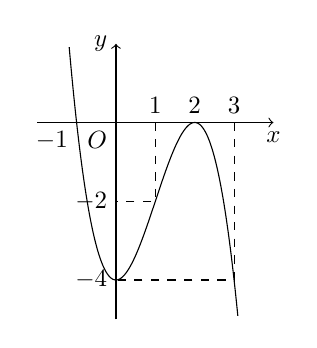
\begin{tikzpicture}[scale=0.5]
            \def\a{-1} \def\b{3} \def\c{0} \def\d{-4} % Hệ số
            \def\xmin{-2} \def\xmax{4}
            \def\ymin{-5} \def\ymax{2}
            %	\draw[color=gray!50,dashed] (\xmin,\ymin) grid (\xmax,\ymax);
            \draw[->] (\xmin,0)--(\xmax,0) node [below]{$x$};
            \draw[->] (0,\ymin)--(0,\ymax) node [left]{$y$};
            \node at (0,0) [below left]{$O$};
            \node at (2,0) [above]{$2$};
            \node at (-1,0) [below left]{$-1$};
            \draw[dashed] (1,0) node [above] {$1$}--(1,-2)--(0,-2) node [left] {$-2$};
            \draw[dashed] (3,0) node [above] {$3$}--(3,-4)--(0,-4) node [left] {$-4$};
            \clip (\xmin+0.1,\ymin+0.1) rectangle (\xmax-0.5,\ymax-0.1);
            \draw[smooth,samples=300][domain=-1.3:3.3] plot(\x,{\a*(\x)^3+\b*(\x)^2+\c*(\x)+\d});
    \end{tikzpicture}}
    \loigiai{
        Ta có $M=\max\limits_{[1;3]} f(x)=f(2)=0$; $m=\min\limits_{[1;3]} f(x)=f(3)=-4$.\\
        nên $M+m=0+(-4)=-4$.
    }
\end{ex}
\begin{ex}%[Dự án tex hóa đề cương Mariecurie - Biên soạn Thầy Nguyễn Ngọc Nguyên]%[2D1K3-1]
    \immini{Cho hàm số $f(x)$ liên tục trên đoạn $[a;b]$ và có đồ thị như hình bên. Gọi $M,m$ lần lượt là giá trị lớn nhất, nhỏ nhất của hàm số $y=|f(x)|$ trên đoạn $[a;b]$. Giá trị của $M-m$ bằng
        \choice[2]
        { \True $4$}
        {$-2$}
        {$5$}
        {$3$}}
    {
        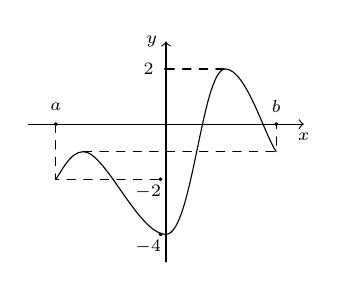
\begin{tikzpicture}[line cap=round, line join=round,font=\scriptsize,y=.7cm,x=.7cm]
            \begin{scope}[scale=.5]
                \draw[->](-5,0)--(5,0)node[below]{$x$};
                \draw[->](0,-5)--(0,3)node[left]{$y$};
                \draw(-4,-2)..controls++(50:0.25) and ++(180:0.5)..(-3,-1)..controls++(0:0.8) and++(180:1)..(0,-4)..controls++(0:0.95) and ++(180:0.85)..(2.15,2)..controls++(0:0.75) and++(125:0.75)..(4,-1);
                \foreach \x/\y/\m/\g in{-4/0/a/90,-0.2/-2/-2/-135,-0.2/-4/-4/-135,4/0/b/90,0/2/2/180}
                \draw[fill=black](\x,\y)circle(1pt)node[shift={(\g:0.35)}]{$\m$};
                \draw[dashed](-4,0)--(-4,-2)--(0,-2)(-3,-1)--(4,-1)--(4,0)(0,2)--(2.15,2);
            \end{scope}
        \end{tikzpicture}
    }
    \loigiai
    {
        Ta vẽ đồ thị hàm $|f(x)|$ bằng cách: Giữ nguyên phần đồ thị nằm phía trên $Ox$ của đồ thị hàm số $f(x)$. Lấy đối xứng phần đồ thị của hàm số $f(x)$ nằm phía dưới $Ox$ qua $Ox$ và xóa phần đồ thị nằm phía dưới $Ox$ của $f(x)$ đi. \\
        Từ đó ta có $M=4$ và $m=0$, do đó $M+m=4$.
    }
\end{ex}
\begin{ex}%[Dự án tex hóa đề cương Mariecurie - Biên soạn Thầy Nguyễn Ngọc Nguyên]%[2D1K3-1]
    \immini{	Cho hàm số $f(x)$ liên tục trên đoạn $[-1;5]$ và có đồ thị như hình vẽ bên. Gọi $M,m$ lần lượt là giá trị lớn nhất, nhỏ nhất của hàm số $y=|f(x)|$ trên đoạn $[-1;5]$. Giá trị của $M-m$ bằng}
    {
        \begin{tikzpicture}[line cap=round, line join=round, scale=0.6]
            \draw[->](-5,0)--(6,0)node[below]{$x$};
            \draw[->](0,-5)--(0,3)node[left]{$y$};
            \draw(-1,-3)..controls++(80:1) and++(180:0.5)..(0,1)..controls++(0:0.5) and++(180:0.75)..(2,-3)..controls++(0:0.5) and++(-100:1)..(3,0)..controls++(80:0.35) and++(180:0.5)..(4,2)..controls++(0:0.5) and++(135:0.25)..(5,1);
            \foreach \x/\y/\m/\g in{-1/0/-1/90,0/-3/-3/-145,2/0/2/90,3/0/3/-70,4/0/4/-90,5/0/5/-90,0/2/2/180}
            \draw[fill=black](\x,\y)circle(1pt)node[shift={(\g:0.35)}]{$\m$};
            \draw[dashed](-1,0)--(-1,-3)--(0,-3)--(2,-3)--(2,0)(0,1)--(5,1)--(5,0)(3,0)--(3,1)(4,0)--(4,2)--(0,2);
        \end{tikzpicture}
    }
    \choice
    {$4$}
    {$2$}
    {\True $3$}
    {$5$}
    \loigiai
    {Ta vẽ đồ thị hàm $|f(x)|$ bằng cách: Giữ nguyên phần đồ thị nằm phía trên $Ox$ của đồ thị hàm số $f(x)$. Lấy đối xứng phần đồ thị của hàm số $f(x)$ nằm phía dưới $Ox$ qua $Ox$ và xóa phần đồ thị nằm phía dưới $Ox$ của $f(x)$ đi. \\
        Từ đó ta có	giá trị lớn nhất và nhỏ nhất của hàm số $y=|f(x)|$ trên $[-1;5]$ lần lượt là $M=3$ và $m=0$.\\ Suy ra $M-m=3$.
    }
\end{ex}
\begin{ex}%[Dự án tex hóa đề cương Mariecurie - Biên soạn Thầy Nguyễn Ngọc Nguyên]%[2D1K3-1]
    \immini{	Cho hàm số $f(x)$ liên tục trên đoạn $[-2;4]$ và có đồ thị như hình vẽ. Gọi $M,m$ lần lượt là giá trị lớn nhất, nhỏ nhất của hàm số $y=f(|x|)$ trên đoạn $[-2;4]$. Giá trị của $M-m$ bằng
        \choice
        { \True $4$}
        {$6$}
        {$7$}
        { $5$}
    }
    {
        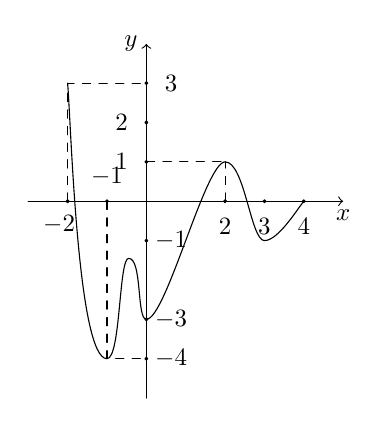
\begin{tikzpicture}[line cap=round, line join=round, scale=0.5]
            \draw[->](-3,0)--(5,0)node[below]{$x$};
            \draw[->](0,-5)--(0,4)node[left]{$y$};
            \draw(-2,3)..controls++(-85:1) and ++(180:0.75)..(-1,-4)..controls++(0:0.35) and++(180:0.25)..(-0.45,-1.45)..controls++(0:0.35) and++(180:0.25)..(0,-3)..controls ++(0:0.5) and++(180:0.5)..(2,1)..controls++(0:0.5)and++(180:0.35)..(3,-1)..controls++(0:0.35) and++(-130:0.25)..(4,0);
            \foreach \x/\y/\m/\g in{0/-4/-4/0,0/-3/-3/0,0/3/3/0,-2/0/-2/-110,-1/0/-1/90,0/-1/-1/0,2/0/2/-90,3/0/3/-90,4/0/4/-90,0/1/1/180,0/2/2/180}
            \draw[fill=black](\x,\y)circle(1pt)node[shift={(\g:0.35)}]{$\m$};
            \draw[dashed](-2,0)--(-2,3)--(0,3)(-1,0)--(-1,-4)--(0,-4)(2,0)--(2,1)(0,1)--(2,1);
        \end{tikzpicture}
    }
    \loigiai
    {Ta vẽ đồ thị của hàm số $y=f(|x|)$ nhứ sau: Giữa nguyên phần đồ thị nằm bên phải trục $Oy$ của hàm số $y=f(x)$, xóa bỏ phần nằm bên trái. Lấy đối xứng phần đồ thị nằm bên phải qua trục Oy.\\
        Từ đó ta có giá trị lớn nhất và nhỏ nhất của hàm số $y=|f(x)|$ trên $[-2;4]$ lần lượt là $M=1$ và $m=-3$.\\ Suy ra $M-m=4$.
    }
\end{ex}
\begin{ex}%[Võ Thị Thùy Trang - DA1]%[2D1G3-2]%7
    \immini
    {Cho hàm số $y=f(x)$ liên tục trên đoạn $[-2;3]$ và có đồ thị như hình vẽ bên dưới. Gọi $M$ và $m$ lần lượt là giá trị lớn nhất và nhỏ nhất của hàm số $y=f\left(2\cos 5x +1\right)$. Giá trị của $M-2m$ bằng
        \choice
        {$10$}
        {$3$}
        {$7$}
        {\True $5$}}
    {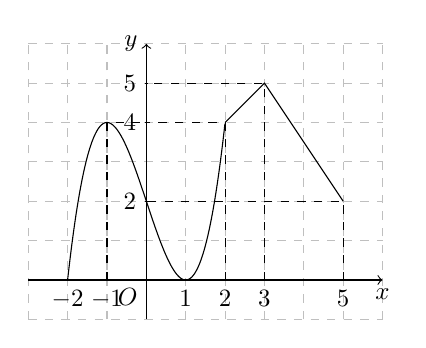
\begin{tikzpicture}[scale=0.5]
            \def\a{1} \def\b{0} \def\c{-3} \def\d{2} % Hệ số
            \def\xmin{-3} \def\xmax{6}
            \def\ymin{-1} \def\ymax{6}
            \draw[color=gray!50,dashed] (\xmin,\ymin) grid (\xmax,\ymax);
            \draw[->] (\xmin,0)--(\xmax,0) node [below]{$x$};
            \draw[->] (0,\ymin)--(0,\ymax) node [left]{$y$};
            \node at (0,0) [below left]{$O$};
            \draw (2,4)--(3,5)--(5,2);
            \draw[dashed] (-1,0)--(-1,4)--(0,4);
            \draw[dashed] (2,0)--(2,4)--(0,4);
            \draw[dashed] (3,0)--(3,5)--(0,5);
            \draw[dashed] (5,0)--(5,2)--(0,2);
            \clip (\xmin+0.1,\ymin+0.1) rectangle (\xmax-0.5,\ymax-0.1);
            \draw[smooth,samples=300][domain=-2:2] plot(\x,{\a*(\x)^3+\b*(\x)^2+\c*(\x)+\d});
            \foreach \x in {-2,-1,1,2,3,5}
            \draw[thin] (\x,1pt)--(\x,-1pt) node [below] {$\x$};
            \foreach \y in {2,4,5}
            \draw[thin] (1pt,\y)--(-1pt,\y) node [left] {$\y$};
    \end{tikzpicture}}
    \loigiai{
        Ta có $-1\le 2\cos 5x +1\le 3$.\\
        Và $M=\max\limits_{[-1;3]} f(x)=f(3)=5$; $m=\min\limits_{[-1;3]} f(x)=f(1)=0$.\\
        Nên $M-2m=5-2(0)=5$.
    }
\end{ex}
\begin{ex}%[Võ Thị Thùy Trang - DA1]%[2D1G3-2]%8
    \immini{Cho hàm số $y=f(x)$ liên tục trên đoạn $[-1;3]$ và có đồ thị như hình vẽ. Giá trị lớn nhất của hàm số $y=f\left(3\sin^2 x -1\right)$ bằng
        \choice
        {$0$}
        {$1$}
        {$3$}
        {\True $2$}
    }
    {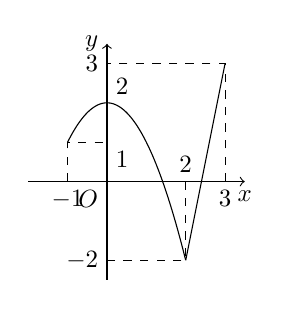
\begin{tikzpicture}[scale=0.5]
            \def\a{-1} \def\b{0} \def\c{2} % Hệ số
            \def\xmin{-2} \def\xmax{3.5}
            \def\ymin{-2.5} \def\ymax{3.5}
            %\draw[color=gray!50,dashed] (\xmin,\ymin) grid (\xmax,\ymax);
            \draw[->] (\xmin,0)--(\xmax,0) node [below]{$x$};
            \draw[->] (0,\ymin)--(0,\ymax) node [left]{$y$};
            \node at (0,0) [below left]{$O$};
            \node at (0,2) [above right]{$2$};
            \draw (2,-2)--(3,3);
            \draw[dashed] (-1,0) node [below] {$-1$}--(-1,1)--(0,1) node [below right] {$1$};
            \draw[dashed] (3,0) node [below] {$3$}--(3,3)--(0,3) node [left] {$3$};
            \draw[dashed] (2,0) node [above] {$2$}--(2,-2)--(0,-2) node [left] {$-2$};
            \clip (\xmin+0.1,\ymin+0.1) rectangle (\xmax-0.5,\ymax-0.1);
            \draw[smooth,samples=300][domain=-1:2] plot(\x,{\a*(\x)^2+\b*(\x)+\c});
    \end{tikzpicture}}
    \loigiai{
        Ta có $-1\le 3\sin^2 x -1\le 2$ nên giá trị lớn nhất của hàm số $y=f\left(3\sin^2 x -1\right)$ bằng $2$.
    }
\end{ex}
\begin{ex}%[Võ Thị Thùy Trang - DA1]%[2D1G3-2]%9
    \immini{Cho hàm số $y=f(x)$ liên tục trên đoạn $[-1;3]$ và có bảng biến thiên bên dưới. Tìm giá trị lớn nhất của hàm số $y=3\left|\cos x\right| -1$.
        \choice
        {$4$}
        {$3$}
        {\True $2$}
        {$1$}
    }
    {
\begin{tikzpicture}[scale=.76,>=stealth, font=\footnotesize, line join=round, line cap=round]
            \tkzTabInit[nocadre=false,lgt=1.2,espcl=2.5,deltacl=0.6]
            {$x$ /0.6, $f'(x)$ /0.6, $f(x)$ /2.5}
            {$-1$,$0$,$2$,$3$}
            \tkzTabLine{,+,$0$,-,$0$,+,}
            \tkzTabVar{-/$1$,+/$2$,-/$-2$,+/$3$}
    \end{tikzpicture}}
    \loigiai{
        Ta có $0\le \left|\cos x\right|\le 1$ nên $-1\le 3\left|\cos x\right| -1\le 2$.\\
        Do đó giá trị lớn nhất của hàm số $y=3\left|\cos x\right| -1$ bằng $2$.
    }
\end{ex}
\begin{ex}%[Võ Thị Thùy Trang - DA1]%[2D1G3-2]%10
    \immini{Cho hàm số $y=f(x)$ liên tục trên đoạn $[-2;2]$ có đồ thị như hình. Gọi $M$, $m$ lần lượt là giá trị lớn nhất và nhỏ nhất của hàm số $y=3f\left(\dfrac{4\sin x -1}{3}\right)$ trên $\left(0;\dfrac{7\pi}{6}\right)$. Giá trị của $2M-m$ bằng
        \choice
        {$4$}
        {\True $2$}
        {$5$}
        {$6$}
    }
    {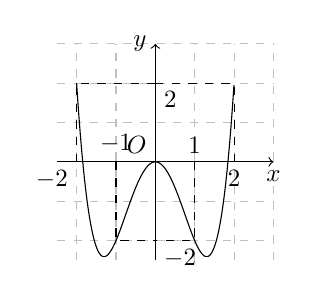
\begin{tikzpicture}[scale=0.5]
            \def\a{5/6} \def\b{-17/6} \def\c{0} % Hệ số
            \def\xmin{-2.5} \def\xmax{3}
            \def\ymin{-2.5} \def\ymax{3}
            \draw[color=gray!50,dashed] (\xmin,\ymin) grid (\xmax,\ymax);
            \draw[->] (\xmin,0)--(\xmax,0) node [below]{$x$};
            \draw[->] (0,\ymin)--(0,\ymax) node [left]{$y$};
            \node at (0,0) [above left]{$O$};
            \draw[dashed] (-2,0) node [below left] {$-2$}--(-2,2)--(0,2) node [below right] {$2$};
            \draw[dashed] (2,0) node [below] {$2$}--(2,2)--(0,2);
            \draw[dashed] (-1,0) node [above] {$-1$}--(-1,-2)--(0,-2) node [below right] {$-2$};
            \draw[dashed] (1,0) node [above] {$1$}--(1,-2)--(0,-2);
            \clip (\xmin+0.1,\ymin+0.1) rectangle (\xmax-0.5,\ymax-0.1);
            \draw[smooth,samples=300][domain=-2:2] plot(\x,{\a*(\x)^4+\b*(\x)^2+\c});
    \end{tikzpicture}}
    \loigiai{Ta có $-\dfrac{1}{2}<\sin x\le 1$, $\forall x\in \left(0;\dfrac{7\pi}{6}\right)$ nên $-1<\dfrac{4\sin x -1}{3}\le 1$.\\
        Do đó $M=0$ và $m=-2$. Vậy $2M-m=2$.
    }
\end{ex}
\begin{ex}%[Võ Thị Thùy Trang - DA1]%[2D1G3-2]%11
    \immini{Cho hàm số $y=f(x)$ liên tục trên đoạn $[-1;3]$ và có đồ thị như hình. Gọi $M$, $m$ lần lượt là giá trị lớn nhất và nhỏ nhất của hàm số $y=f\left(f(x)\right)$ trên đoạn $\left[-1;0\right]$. Giá trị của $M-m$ bằng
        \choice
        {$2$}
        {\True $3$}
        {$4$}
        {$5$}
    }
    {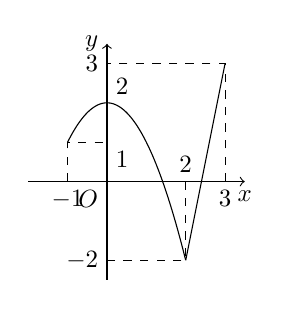
\begin{tikzpicture}[scale=0.5]
            \def\a{-1} \def\b{0} \def\c{2} % Hệ số
            \def\xmin{-2} \def\xmax{3.5}
            \def\ymin{-2.5} \def\ymax{3.5}
            %\draw[color=gray!50,dashed] (\xmin,\ymin) grid (\xmax,\ymax);
            \draw[->] (\xmin,0)--(\xmax,0) node [below]{$x$};
            \draw[->] (0,\ymin)--(0,\ymax) node [left]{$y$};
            \node at (0,0) [below left]{$O$};
            \node at (0,2) [above right]{$2$};
            \draw (2,-2)--(3,3);
            \draw[dashed] (-1,0) node [below] {$-1$}--(-1,1)--(0,1) node [below right] {$1$};
            \draw[dashed] (3,0) node [below] {$3$}--(3,3)--(0,3) node [left] {$3$};
            \draw[dashed] (2,0) node [above] {$2$}--(2,-2)--(0,-2) node [left] {$-2$};
            \clip (\xmin+0.1,\ymin+0.1) rectangle (\xmax-0.5,\ymax-0.1);
            \draw[smooth,samples=300][domain=-1:2] plot(\x,{\a*(\x)^2+\b*(\x)+\c});
    \end{tikzpicture}}
    \loigiai{
        Ta có $1\le f(x)\le 2$, $\forall x\in \left[-1;0\right]$.\\
        Và	$\max\limits_{[1;2]} f(x)=f(1)=1$, $\min\limits_{[1;2]} f(x)=f\left(2\right)=-2$.\\
        Suy ra $M=\max\limits_{[-1;0]} f(f(x))=1$, $m=\min\limits_{[-1;0]} f(f(x))=-2$.\\
        Do đó $M-m=1-(-2)=3$.
    }
\end{ex}
\begin{ex}%[Võ Thị Thùy Trang - DA1]%[2D1G3-2]%12
    \immini{Cho hàm số $y=f(x)$ xác định, liên tục trên đoạn $[-2;2]$ và có đồ thị là đường cong trong hình vẽ bên dưới. Gọi $M$, $m$ lần lượt là giá trị lớn nhất và nhỏ nhất của hàm số $y=f\left(f(x)\right)$ trên đoạn $\left[-1;1\right]$. Giá trị của $M-m$ bằng
        \choice
        {$2$}
        {$4$}
        {$6$}
        {\True $8$}
    }
    {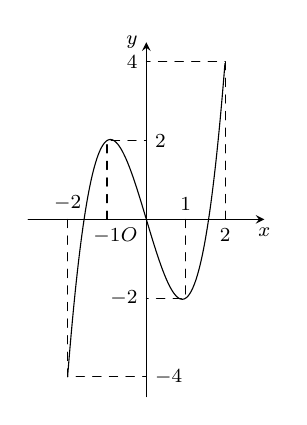
\begin{tikzpicture}[scale=.5,>=stealth, font=\footnotesize, line join=round, line cap=round]
            \def\a{4/3} \def\b{0} \def\c{-10/3} \def\d{0} % Hệ số
            \def\xmin{-3} \def\xmax{3}
            \def\ymin{-4.5} \def\ymax{4.5}
            %	\draw[color=gray!50,dashed] (\xmin,\ymin) grid (\xmax,\ymax);
            \draw[->] (\xmin,0)--(\xmax,0) node [below]{$x$};
            \draw[->] (0,\ymin)--(0,\ymax) node [left]{$y$};
            \node at (0,0) [below left]{$O$};
            \draw[dashed] (-2,0) node [above] {$-2$}--(-2,-4)--(0,-4) node [right] {$-4$};
            \draw[dashed] (-1,0) node [below] {$-1$}--(-1,2)--(0,2) node [right] {$2$};
            \draw[dashed] (1,0) node [above] {$1$}--(1,-2)--(0,-2) node [left] {$-2$};
            \draw[dashed] (2,0) node [below] {$2$}--(2,4)--(0,4) node [left] {$4$};
            \clip (\xmin+0.1,\ymin+0.1) rectangle (\xmax-0.5,\ymax-0.1);
            \draw[smooth,samples=300][domain=-2:2] plot(\x,{\a*(\x)^3+\b*(\x)^2+\c*(\x)+\d});
    \end{tikzpicture}}
    \loigiai{
        Ta có $-2\le f(x)\le 2$, $\forall x\in \left[-1;1\right]$.\\
        Và	$\max\limits_{[-2;2]} f(x)=f(2)=4$, $\min\limits_{[-2;2]} f(x)=f\left(-2\right)=-4$.\\
        Suy ra $M=\max\limits_{[-1;1]} f(f(x))=4$, $m=\min\limits_{[-1;1]} f(f(x))=-4$.\\
        Do đó $M-m=4-(-4)=8$.
    }
\end{ex}
%Câu 57
\begin{ex}%[2D1K3-1]%[Dự án TEX hóa đề cương Marie Curie - Ân Trương]
    \immini
    {
        Cho hàm số $ y=f(x) $ có đạo hàm liên tục trên đoạn $ \left [0;\dfrac{7}{2}\right ] $ và đồ thị hàm số $ y=f'(x) $ như hình vẽ. Khi đó hàm số $ y=f(x) $ đạt giá trị nhỏ nhất trên đoạn $ \left [0;\dfrac{7}{2}\right ] $ tại điểm $ x_0 $ nào dưới đây ?
        \choice
        {$x_0=2$}
        {$x_0=1$}
        {$x_0=0$}
        {\True$x_0=3$}
    }
    {
        \begin{tikzpicture}[>=stealth, samples=100,smooth,y=.7cm,font=\scriptsize]
            \begin{scope}[scale=.7]
                \draw[->] (-1,0)--(4.5,0) node[below] {$x$};
                \draw[->] (0,-2)--(0,4) node[right] {$y$};
                \draw (0,0) node [below left] {$O$};
                \draw[dashed] (3.6,0)--(3.6,4);
                \draw[samples=200,domain=0.2:3.6,smooth,variable=\x]
                plot (\x,{1.06*(\x)^3-5.3*(\x)^2+7.23*(\x)-3});
                \path
                (3.6,0)node[below]{$\dfrac{7}{2}$}
                (3,0)node[above left]{$3$}
                (1,0)node[above]{$1$}
                ;
            \end{scope}
        \end{tikzpicture}
    }
    \loigiai{
        Tập xác định $ \mathscr{D} = \left [0;\dfrac{7}{2}\right ]$.\\
        Dựa vào đồ thị, cho $ f'(x)=0 \Leftrightarrow\hoac{& x=1 \\ & x=3.}$\\
        Ta có bảng biến thiên của hàm số $ y=f(x) $
        \begin{center}
            
\begin{tikzpicture}
                \tkzTabInit[nocadre=false,lgt=1.2,espcl=2.5,deltacl=0.6]
                {$x$ /1,$f’(x)$ /1,$f(x)$ /2}
                {$0$,$3$,$\dfrac{7}{2}$}
                \tkzTabLine{,-,0,+,}
                \tkzTabVar{+/ ,-/$f(3)$,+/ }
            \end{tikzpicture}
        \end{center}
        Dựa vào bảng biến thiên, hàm số $y=f(x) $ tại giá trị nhỏ nhất trên $ \left [0;\dfrac{7}{2}\right ] $ tại $ x_0=3 $.
    }
\end{ex}
\begin{ex}%Câu 4%[Phat Dang Tan - DA1]%[2D1K3-1]
    Cho hàm số $y=f(x)$ xác định và liên tục trên $[-2;2]$, có đồ thị $y=f'(x)$ như hình vẽ bên dưới. Tìm giá trị $x_0$ để hàm số $y=f(x)$ đạt giá trị lớn nhất trên $[-2;2]$.
    \begin{center}
        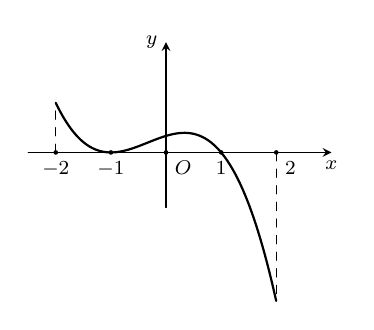
\begin{tikzpicture}[>=stealth,line join=round,line cap=round,font=\footnotesize,scale=0.7]
            \draw[->] (-2.5,0)--(3,0) node[below]{$x$};
            \draw[->] (0,-1)--(0,2) node[left]{$y$};
            \fill[name=O] (0,0) circle (1.2pt) node[below right]{$O$};
            \coordinate[label=below:{$1$}] (a) at (1,0);
            \coordinate[label=below:{$-1$}] (b) at (-1,0);
            \coordinate[label=below:{$-2$}] (c) at (-2,0);
            \coordinate[label=below right:{$2$}] (d) at (2,0);
            %\coordinate (d) at (3/2,1);
            \draw[dashed] (-2,0)|-(-2,9/10);
            \draw[dashed] (2,0)|-(2,-27/10);
            \draw[color=black,thick, smooth, samples=100, domain= -2:2] plot(\x,{-3/10*(\x)^3-3/10*(\x)^2+3/10*\x+3/10});
            \foreach \point in {a,b,c,d}
            \fill (\point) circle (1.2pt);
        \end{tikzpicture}
    \end{center}
    \choice
    {$2$}
    {$-1$}
    {$-2$}
    {\True $1$}
    \loigiai{
        Xét trên $[-2;2]$ ta có $y'=0\Leftrightarrow \hoac{&x=-1\\&x=1.}$	\\
        Bảng biến thiên
        \begin{center}
            \begin{tikzpicture}
                \tkzTabInit[lgt=1.2,espcl=2.5,deltacl=0.6]
                {$t$ /0.6,$f'(x)$ /0.6,$f(x)$ /2}
                {$-2$,$-1$,$1$,$2$}
                \tkzTabLine{,+,$0$,+,$0$,-}
                \node (0) at ($(N13)+(0,.2)$){$f(-2)$};
                \node (1) at ($(N32)-(0,.3)$){$f(1)$};
                \node (2) at ($(N43)+(0,.2)$){$f(2)$};
                \draw[-stealth] (0)--(1);
                \draw[-stealth] (1)--(2);
            \end{tikzpicture}
        \end{center}
        Suy ra $\max\limits_{[-2;2]} y=f(1)$ khi $x=1$.
    }
\end{ex}
%Câu 58
\begin{ex}%[2D1K3-1]%[Dự án TEX hóa đề cương Marie Curie - Ân Trương]
    \immini
    {
        Cho hàm số $ y=f(x) $ có đạo hàm liên tục trên đoạn $ [-1;2] $ và đồ thị hàm số $ y=f'(x) $ như hình vẽ. Gọi $ M $ là giá trị lớn nhất của hàm số $ y=f(x) $ trên đoạn $ [-1;2] $. Mệnh đề nào dưới đây đúng?
        \choice
        {$M=\max \left\{f\left(-\dfrac{1}{2}\right) ; f(1) ; f\left(\dfrac{5}{3}\right)\right\}$}
        {\True$M=\max \{f(-1) ; f(1) ; f(2)\}$}
        {$M=f(0)$}
        {$M=f(2)$}
    }
    {
        \begin{tikzpicture}[>=stealth,x=1cm,y=1cm,scale=0.9,font=\footnotesize]
            \path
            (0,0) coordinate (O)
            (3,0) coordinate (Bf)
            (-1.2,0) coordinate (Af)
            (0,0) coordinate (O)node[above right]{$ O $}
            (-1.2,-1.6) coordinate (P)
            (0,1.2) coordinate (D)node[shift={(1,0.1)}]{$ y=f'(x)$}
            (2.3,-0.6) coordinate (Q)
            (3,1.9) coordinate (M)
            ;
            %	\draw[red] (P)--(D)--(Q)--(M);
            \draw[name path=ox] (Af)--(Bf);
            \draw[name path=fx,thick,black]
            (P)..controls +(80:0.5) and+(-175:0.6)..
            (D)..controls +(-10:0.5) and+(170:0.45)..(Q)
            ..controls +(10:0.5) and+(-100:0.25)..(M)
            ;
            \path[name intersections={of=fx and ox, by={A,B1,B2}}] ;
            %Vẽ hệ trục tọa dộ:
            \draw[->] (-1.7,0)--(0,0)--(3.5,0) node[below]{$x$};
            \draw[->] (0,-1.8) --(0,2.5) node[left]{$y$};
            %	Node các điểm
            \foreach \p in {A,B1,B2,M,P,O}
            \fill (\p) circle (1.5pt) ;
            %	Vẽ nét đứt+node:
            \foreach \p/\n/\r in {P/-1/90,A/-\frac{1}{2}/-60,B1/1/90,B2/\frac{5}{3}/100,M/2/-90}
            \draw[dashed](\p)--($(Af)!(\p)!(Bf)$)node[shift={(\r:3mm)}]{$ \n $} ;
        \end{tikzpicture}
    }
    \loigiai{
        Tập xác định $ \mathscr{D} = [-1;2]$.\\
        Dựa vào đồ thị, cho $ f'(x)=0 \Leftrightarrow\hoac{& x=-\dfrac{1}{2} \\ & x=1 \\&x=\dfrac{5}{3}.}$\\
        Ta có bảng biến thiên của hàm số $ y=f(x) $
        \begin{center}
            
\begin{tikzpicture}
                \tkzTabInit[nocadre=false,lgt=1.2,espcl=2.5,deltacl=0.7]
                {$x$ /1,$y’$ /1,$y$ /3}
                {$-1$,$-\dfrac{1}{2}$,$1$,$\dfrac{5}{3}$,$2$}
                \tkzTabLine{,-,0,+,0,-,0,+,}
                \tkzTabVar{+/$f(-1)$,-/$f\left (-\dfrac{1}{2}\right )$,+/$f(1)$,-/$f\left (\dfrac{5}{3}\right )$,+/$f(2)$}
            \end{tikzpicture}
        \end{center}
        Dựa vào bảng biến thiên, ta thấy $M=\max \left \{f(-1) ; f(1) ; f(2)\right \}$.
    }
\end{ex}
\BTTF
\begin{ex}%[2D1N3-2]%[Dự án EX-TF-TLN-2024 - Đợt 1]%[Thành Đức Trung]
    Cho hàm số $y=f(x)$ trên khoảng $K$.
    \choiceTF
    {\True Giá trị lớn nhất của $f(x)$ trong khoảng $K$ là $M$ khi và chỉ khi $ \heva{f(x) \le M \text{ với } \forall x \in K \\ \exists x_0 \in K \text{ để } f(x_0)=M}$}
    {\True Nếu hàm số $f(x)$ đạt giá trị lớn nhất $M$ trong khoảng $K$ thì có thể tổn tại nhiều giá trị của $x_0 \in K$ sao cho $f(x_0)=M$}
    {$\mathop {\min }\limits_{K} \,\,f(x) = m \Leftrightarrow f(x) \ge m \hspace{0.3cm} \forall x \in K$}
    {Có thể tồn tại nhiều giá trị nhỏ nhất của $f(x)$ trên khoảng $K$}
    \loigiai{
        \begin{itemchoice}
            \itemch \textbf{Đúng}.
            \itemch \textbf{Đúng}.
            \itemch \textbf{Sai}. Chiều suy ra thì đúng nhưng chiều ngược lại chưa chắc chắn, phải chỉ ra tồn tại $x_0$ thuộc $K$ để $f(x_0) = m$.
            \itemch \textbf{Sai}. Vì nếu giá trị nhỏ nhất của hàm số tồn tại thì duy nhất.
        \end{itemchoice}
    }
\end{ex}
\begin{ex}%[Dự án tex hóa đề cương Mariecurie - Biên soạn Thầy Nguyễn Ngọc Nguyên]%[2D1B3-2]
    Hàm số $y=f(x)$ liên tục trên $\mathbb{R}$ và có bảng biến thiên như hình bên.
    \begin{center}
        
\begin{tikzpicture}
            \tkzTabInit[espcl=3]
            {$x$ /.7, $y'$ /.7,$y$ /2}
            {$-\infty$, $-2$, $1$, $7$, $+\infty$}
            \tkzTabLine{,-,d, +, $0$, -, d ,-,}
            \tkzTabVar{ +/$3$,-/$-4$,+/$1$,R/, -/$-4$}
            \tkzTabIma{3}{5}{4}{$-3$}
        \end{tikzpicture}
    \end{center}
    Xét tính đúng, sai của các khẳng định sau đây
    \choiceTF
    {Hàm số có giá trị lớn nhất bằng $3$}
    {Hàm số có giá trị nhỏ nhất bằng $-3$}
    {Hàm số có giá trị lớn nhất bằng $1$}
    {\True Hàm số có giá trị nhỏ nhất bằng $-4$}
    \loigiai
    {Dựa vào bảng biến thiên ta thấy hàm số đạt giá trị nhỏ nhất bằng $-4$ tại $x=-2$.
    }
\end{ex}
\begin{ex}%[Dự án tex hóa đề cương Mariecurie - Biên soạn Thầy Nguyễn Ngọc Nguyên]%[2D1B3-2]
    Hàm số $y=f(x)$ liên tục trên $\mathbb{R}$ và có bảng biến thiên như hình bên.
    \begin{center}
        
\begin{tikzpicture}
            \tkzTabInit[espcl=3]
            {$x$ /.7, $y'$ /.7,$y$ /2}
            {$-\infty$,$0$,$1$,$+\infty$}
            \tkzTabLine{,+,d ,-,$0$,+}
            \tkzTabVar{ -/$-3$,+/$2$,-/$-2$,+/$1$}
        \end{tikzpicture}
    \end{center}
    Xét tính đúng, sai của các mệnh đề sau
    \choiceTF
    { Giá trị nhỏ nhất của hàm số bằng $-2$}
    {Giá trị nhỏ nhất của hàm số bằng $-3$}
    {Giá trị lớn nhất của hàm số bằng $1$}
    { \True Giá trị lớn nhất của hàm số bằng $2$}
    \loigiai
    {Dựa vào bảng biến thiên ta thấy hàm số đạt giá trị lớn nhất bằng $2$ tại $x=0$.
    }
\end{ex}
\begin{ex}%[Dự án tex hóa đề cương Mariecurie - Biên soạn Thầy Nguyễn Ngọc Nguyên]%[2D1B3-2]
    Cho hàm số $y=f(x)$ liên tục trên $(-\infty; 2]$ và có bảng biến thiên như hình bên.
    \begin{center}
        \begin{tikzpicture}
            \tkzTabInit[nocadre=false,lgt=1,espcl=1.8]
            {$x$ /0.9,$y'$ /0.7,$y$ /2}
            {$-\infty$,$-1$,$2$,}
            \tkzTabLine{,-,$0$,+ , d,h, }
            \tkzTabVar{+/ $4$,-/$3$/, +CH/ /	}
            \draw[draw=none,pattern=north west lines](N41) rectangle (T23);
            %	\draw[draw=none,pattern=north west lines](N11) rectangle (T13);
        \end{tikzpicture}
    \end{center}
    Xét tính đúng, sai của các câu sau
    \choiceTF
    {\True$y_\text{CT}=3$}
    { $y_\text{CĐ}=5$}
    {\True$\min\limits{(-\infty; 2]}=3$}
    {\True$\max\limits{(-\infty; 2]}=5$}
    \loigiai{
        Từ bảng biến thiên ta thấy hàm số không có cực đại trên $(-\infty; 2]$. Nên khẳng định \lq\lq $y_\text{CĐ}=5$ \rq\rq \,là khẳng định sai.
    }
\end{ex}
\begin{ex}%[2D1B3-1]
    Cho hàm số $y=f(x)$ có bảng biến thiên như hình vẽ
    \begin{center}
        
\begin{tikzpicture}[>=stealth]
            \tkzTabInit[nocadre=false,lgt=1,espcl=3,deltacl=0.5]{$x$/.7 ,$y'$/.7,$y$/2}
            {$-\infty$ , $-1$ , $+\infty$}
            \tkzTabLine{ , + , d , + , }
            \tkzTabVar{-/$2$ , +D-/$+\infty$/$-\infty$ , +/$5$}
        \end{tikzpicture}
    \end{center}
    Xét tính đúng, sai của các khẳng định sau
    \choiceTF
    {Hàm số có max trên $(-\infty;-1)$}
    {\True Hàm số có min trên $[2;+\infty)$}
    {Hàm số không có min trên $[0;2]$}
    {Hàm số có max và min trên $[-2;1]$}
\end{ex}
\begin{ex}%[2D1B3-2]
    Cho hàm số $y=f(x)$ có bảng biến thiên như hình vẽ.
    \begin{center}
        
\begin{tikzpicture}[>=stealth]
            \tkzTabInit[nocadre=false,lgt=1,espcl=3,deltacl=0.5]{$x$/.7 ,$y'$/.7,$y$/2}
            {$-\infty$ , $-1$,$0$,$1$ , $+\infty$}
            \tkzTabLine{ , + , d , - ,0,+,d,- }
            \tkzTabVar{-/$-\infty$ ,+/$1$,-/$-1$,+D+/$+\infty$/$+\infty$ , -/$-\infty$}
        \end{tikzpicture}
    \end{center}
    Xét tính đúng, sai của các mệnh đề sau
    \choiceTF
    {Hàm số có ba cực trị}
    {\True Hàm số đạt cực đại tại $x=-1$}
    {Hàm số có max bằng $1$ và min bằng $-1$}
    {Hàm số đạt cực tiểu tại $x=-1$}
\end{ex}
\begin{ex}%[2D1H3-1]%[GV- Thái Văn Sang]%[Du-An-Ngan-Hang-Cau-Hoi-2024-K12]%6
    \immini{
        Cho hàm số $y = f(x)$ liên tục trên đoạn $[-1;3]$ có đồ thị như hình vẽ. Xét tính đúng hoặc sai của các phát biểu sau
        \choiceTF
        {\True Giá trị lớn nhất của hàm số trên đoạn $[-1;3]$ bằng $3$}
        {\True Giá trị nhỏ nhất của hàm số trên đoạn $[-1;3]$ bằng $-2$}
        {\True Giá trị lớn nhất của hàm số trên đoạn $[-1;2]$ bằng $2$}
        {Giá trị nhỏ nhất của hàm số trên đoạn $[1;2]$ bằng $-2$}
    }{
        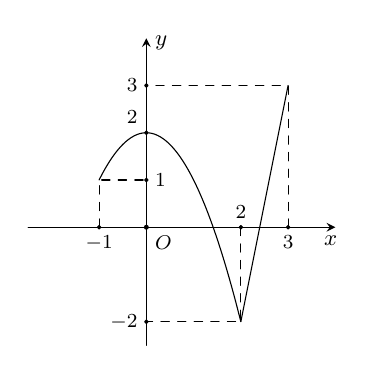
\begin{tikzpicture}[scale=0.6, font=\footnotesize, line join=round, line cap=round, >=stealth]
            %\clip(- 3,- 4) rectangle (4, 4);
            \draw[->] (-2.5,0) -- (4,0);\draw (3.9,0) node[below] {\small $x$};
            \draw[->] (0,-2.5) -- (0,4);\draw (0,3.9) node[right] {\small $y$};
            \draw[fill=black] (-1,0) node[below]{$-1$} circle (1pt);
            \draw[fill=black] (2,0) node[above]{$2$} circle (1pt);
            \draw[fill=black] (3,0) node[below]{$3$} circle (1pt);
            \draw[fill=black] (0,3) node[left]{$3$} circle (1pt);
            \draw[fill=black] (0,2) node[above left]{$2$} circle (1pt);
            \draw[fill=black] (0,1) node[right]{$1$} circle (1pt);
            \draw[fill=black] (0,-2) node[left]{$-2$} circle (1pt);
            \draw plot[domain=-1:2, samples=100] (\x,{2-(\x)^2});
            \draw(2,-2)--(3,3);
            \fill (0,0) node[below right]{$O$} circle (1.5pt);
            \draw[dashed] (-1,0)--(-1,1)--(0,1);
            \draw[dashed] (2,0)--(2,-2)--(0,-2);
            \draw[dashed] (3,0)--(3,3)--(0,3);
        \end{tikzpicture}
    }
    \loigiai{
        Dựa vào đồ thị ta có
        \begin{itemchoice}
            \itemch{\bf Đúng}. Vì giá trị lớn nhất của hàm số trên đoạn $[-1;3]$ bằng $3$.
            \itemch {\bf Đúng}. Vì giá trị nhỏ nhất của hàm số trên đoạn $[-1;3]$ bằng $-2$.
            \itemch {\bf Đúng}. Vì giá trị lớn nhất của hàm số trên đoạn $[-1;2]$ bằng $2$.
            \itemch {\bf Đúng}. Vì trên đoạn $[-1;2]$ hàm số đạt giá trị nhỏ nhất bằng $-2$ tại điểm $x=2$.
        \end{itemchoice}
    }
\end{ex}
\begin{ex}%[2D1H3-1]%[GV- Thái Văn Sang]%[Du-An-Ngan-Hang-Cau-Hoi-2024-K12]%10
    \immini{Cho hàm số $y=f(x)$ liên tục trên $R$ và hàm số $y=f'(x)$ có đồ thị như hình vẽ dưới đây.Xét hàm số $y=f(x)$ trên đoạn $\left[\dfrac{1}{2};\dfrac{3}{2} \right]$, biết $f\left(\dfrac{3}{2}\right)<f\left(\dfrac{1}{2}\right)$. Xét tính đúng hoặc sai của các phát biểu sau đây?
        \choiceTF
        { Hàm số $y=f(x)$ đạt giá trị lớn nhất trên đoạn $\left[\dfrac{1}{2};\dfrac{3}{2} \right]$ tại $x=\dfrac{3}{2}$}
        {\True Hàm số $y=f(x)$ đạt giá trị lớn nhất trên đoạn $\left[\dfrac{1}{2};\dfrac{3}{2} \right]$ tại $x=\dfrac{1}{2}$}
        { \True Hàm số $y=f(x)$ đạt giá trị nhỏ nhất trên đoạn $\left[\dfrac{1}{2};\dfrac{3}{2} \right]$ tại $x=1$}
        {Hàm số $y=f(x)$ đạt giá nhỏ lớn nhất trên đoạn $\left[\dfrac{1}{2};\dfrac{3}{2} \right]$ tại $x=\dfrac{1}{2}$}}
    {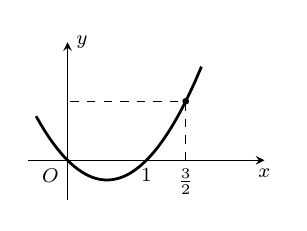
\begin{tikzpicture}[>=stealth,scale=1,font=\footnotesize]
            \draw[->] (-0.5,0)--(2.5,0) node[below]{ $x$};
            \draw[->] (0,-0.5)--(0,1.5) node[right]{\footnotesize $y$};
            \draw (0,0) node[below left]{\footnotesize $O$};
            \draw[line width = 1pt,black,smooth,domain=-0.4:1.7] plot({\x},{(\x)^2-\x});
            \draw[fill=black] (1.5,0.75) circle(1pt);
            \draw [dashed] (1.5,0)
            node[below]{\footnotesize$\frac{3}{2}$}--(1.5,0.75)--(0,0.75)(1,0)node[below]{$1$};
        \end{tikzpicture}
    }
    \loigiai{
        Dựa vào đồ thị hàm số $y=f'(x)$. Ta có bảng biến thiên
        \begin{center}
            
\begin{tikzpicture}
                \tkzTabInit[nocadre=false, lgt=1, espcl=2.5]{$x$ /1,$y'$ /1,$y$ /2}{$\dfrac{1}{2}$,$1$,$\dfrac{3}{2}$}
                \tkzTabLine{,-,$0$,+,}
                \tkzTabVar{+/$f(\frac{1}{2})$ ,-/$f(1)$,+/$f(\frac{3}{2})$}
            \end{tikzpicture}
        \end{center}
        \noindent Suy ra hàm số đạt giá trị nhỏ nhất trên $\left[\dfrac{1}{2};\dfrac{3}{2} \right]$ tại $x=1$.\\
        Do $f(\frac{3}{2})<f(\frac{1}{2})$ nên hàm số đạt giá trị lớn nhất trên $\left[\dfrac{1}{2};\frac{3}{2} \right]$ tại $x=\dfrac{1}{2}$.\\
        Nên ta có các kết luận sau
        \begin{itemchoice}
            \itemch{\bf{Sai}}. Vì dựa vào bảng biến thiên và điều kiện $f(\frac{3}{2})<f(\frac{1}{2})$ nên $\max\limits_{x \in [\frac{1}{2} ; \frac{3}{2}]} f(x)=f(\frac{1}{2})$.
            \itemch {\bf{Đúng}}. Vì dựa vào bảng biến thiên và điều kiện $f(\frac{3}{2})<f(\frac{1}{2})$ nên $\max\limits_{x \in [\frac{1}{2} ; \frac{3}{2}]} f(x)=f(\frac{1}{2})$.
            \itemch {\bf{Đúng}}. Vì dựa vào bảng biến thiên và điều kiện $f(\frac{3}{2})<f(\frac{1}{2})$ nên $\min\limits_{x \in [\frac{1}{2} ; \frac{3}{2}]} f(x)=f(1)$.
            \itemch {\bf{Sai}}. Vì tại $a=\dfrac{1}{2}$ thì hàm số đạt giá trị lớn nhất.
        \end{itemchoice}
    }
\end{ex}
\begin{ex}%[2D1V3-1]%[GV- Thái Văn Sang]%[Du-An-Ngan-Hang-Cau-Hoi-2024-K12]%10
    \immini{ Cho hàm số $f(x)$ có đồ thị của hàm số $y=f'(x)$ như hình vẽ. Biết $f(0)+f(1)-2f(2)=f(4)-f(3)$. Gọi giá trị nhỏ nhất $m$, giá trị lớn nhất $M$ của hàm số $f(x)$ trên đoạn $[0;4]$. Xét tính đúng hoặc sai của các phát biểu sau
        \choiceTF
        {\True $M=f(2)$}
        {\True $m=f(4)$}
        {$m=f(-1)$}
        {$M=f(1)$}
    }{
        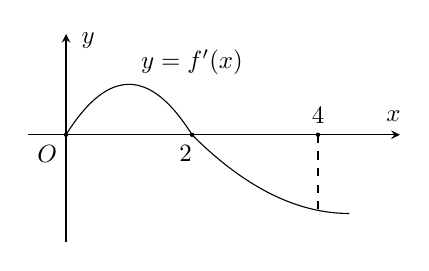
\begin{tikzpicture}[scale=0.8, >=stealth]
            \draw[->] (-0.6,0.) -- (5.3,0.);
            \draw[->] (0.,-1.7) -- (0.,1.6);
            \draw[dashed] (4,0) -- (4,-1.2);
            \clip(-0.6,-1.7) rectangle (5.3,1.7);
            \draw[smooth,samples=100,domain=0:2] plot(\x,{-0.8*((\x)^2-2*(\x))});
            \draw[smooth,samples=100,domain=2:4.5] plot(\x,{0.2*(((\x)-2)*((\x)-7)});
            \draw (-0.3,-0.3) node {$O$} (5.2,0.3) node {$x$} (0.35,1.5) node {$y$} (1.9,-0.3) node {$2$} (4.0,0.3) node {$4$} (2.0,1.15) node {$y=f'(x)$};
            \fill (0,0) circle(1pt) (2,0) circle(1pt) (4,0) circle(1pt);
        \end{tikzpicture}
    }
    \loigiai{
        Từ đồ thị hàm số $y=f'(x)$ ta suy ra $f'(x)=0 \Leftrightarrow \hoac{&x=0\\&x=2.}$\\
        Ta có bảng biến thiên
        \begin{center}
\begin{tikzpicture}[>=stealth,scale=1]
                \tkzTabInit[lgt=1.2,espcl=2.5]
                {$x$/1,$f'(x)$/1,$f(x)$/2.5}
                {$0$,$2$,$4$}
                \tkzTabLine{$0$,+,$0$,- }
                \tkzTabVar{-/$f(0)$,+/$f(2)$,-/$f(4)$}
        \end{tikzpicture}\end{center}
        Từ bảng biến thiên ta thấy $M=f(2)$.\\
        Mặt khác, từ bảng biến thiên ta có $\heva{&f(1)<f(2)\\&f(3)<f(2)}\Rightarrow f(1)+f(3)<2f(2)$.\\
        Do đó $f(4)=f(0)+f(1)+f(3)-2f(2)<f(0)+f(2)+f(2)-2f(2)=f(0) \Rightarrow m=f(4)$.
        \begin{itemchoice}
            \itemch{\bf{Đúng}}. Vì $M=f(2)$.
            \itemch {\bf{Đúng}}. Vì $m=f(4)$.
            \itemch {\bf{Sai}}. Vì $m=f(4)$.
            \itemch {\bf{Sai}}. Vì $M=f(2)$.
        \end{itemchoice}
    }
\end{ex}
\BTTL
\begin{ex}
    Tìm giá trị lớn nhất và giá trị nhỏ nhất của hàm số có đồ thị như hình vẽ sau
    \begin{listEX}[3]
        \item
        \begin{tikzpicture}[line join=round, line cap=round,>=stealth,thick,scale=0.8]
            \tikzset{every node/.style={scale=0.9}}
            \draw[->] (-2.1,0)--(4.1,0) node[below left] {$x$};
            \draw[->] (0,-1.1)--(0,5.1) node[below left] {$y$};
            \draw (0,0) node [below left] {$O$};
            \foreach \x/\nx in {-1/-1,3/3}
            \draw[thin] (\x,1pt)--(\x,-1pt) node [below] {$\nx$};
            \foreach \y/\ny in {1/1,0.5/0.5,4.5/\dfrac{9}{2}}
            \draw[thin] (1pt,\y)--(-1pt,\y) node [right] {$\ny$};
            \draw[dashed,thin](3,0)--(3,4.5)--(0,4.5);
            \draw[dashed,thin] (-1,0)--(-1,0.5)--(0,0.5);
            \node[red,rotate=70] at (2,3.5){$y=f(x)$};
            \begin{scope}
                \clip (-1,-1) rectangle (4,5);
                \draw[red, samples=200,domain=-2:3,smooth,variable=\x] plot (\x,{0.5*(\x)^2+0*(\x)+0});
            \end{scope}
        \end{tikzpicture}
        \item
        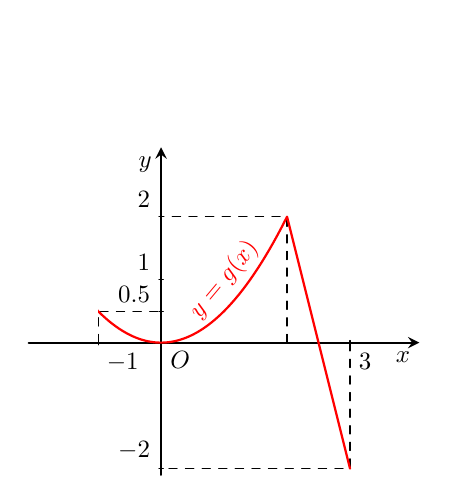
\begin{tikzpicture}[line join=round, line cap=round,>=stealth,thick,scale=0.8]
            \tikzset{every node/.style={scale=0.9}}
            \draw[->] (-2.1,0)--(4.1,0) node[below left] {$x$};
            \draw[->] (0,-2.1)--(0,3.1) node[below left] {$y$};
            \draw (0,0) node [below right] {$O$};
            \foreach \x/\nx in {-1/-1,3/3}
            \draw[thin] (\x,1pt)--(\x,-1pt) node [below right] {$\nx$};
            \foreach \y/\ny in {1/1,2/2,0.5/0.5,-2/-2}
            \draw[thin] (1pt,\y)--(-1pt,\y) node [above left] {$\ny$};
            \draw[dashed,thin](2,0)--(2,2)--(0,2);
            \draw[dashed,thin] (-1,0)--(-1,0.5)--(0,0.5);
            \draw[dashed,thin] (3,0)--(3,-2)--(0,-2);
            \draw[red] (2,2)--(3,-2);
            \node[red,rotate=50] at (1,1){$y=g(x)$};
            \begin{scope}
                \clip (-1,-1) rectangle (4,5);
                \draw[red, samples=200,domain=-2:2,smooth,variable=\x] plot (\x,{0.5*(\x)^2+0*(\x)+0});
            \end{scope}
        \end{tikzpicture}
        \item
        \begin{tikzpicture}[line join=round, line cap=round,>=stealth,thick,scale=0.8,font=\footnotesize]
            \tikzset{every node/.style={scale=0.9}}
            \draw[->] (-2.1,0)--(4.1,0) node[below left] {$x$};
            \draw[->] (0,-2.1)--(0,4.1) node[below left] {$y$};
            \draw (0,0) node [below left] {$O$};
            \foreach \x/\nx in {-1/-1,3/3,1/1,2/2}
            \draw[thin] (\x,1pt)--(\x,-1pt) node [below left] {$\nx$};
            \foreach \y/\ny in {-1/-1,1/1,2/2,3/3,0.5/0.5,-2/-2,2.5/\frac{5}{2},-1.5/\frac{-3}{2}}
            \draw[thin] (1pt,\y)--(-1pt,\y) node [left] {$\ny$};
            \draw[dashed,thin](-1,0)--(-1,2.5)--(0,2.5);
            \draw[dashed,thin] (3,0)--(3,-1.5)--(0,-1.5);
            \node[red,rotate=0] at (1,1){$y=h(x)$};
            \begin{scope}
                \clip (-3,-3) rectangle (4,5);
                \draw[red, samples=200,domain=-1:3,smooth,variable=\x] plot (\x,{-0.5*(\x)^2+0*(\x)+3});
            \end{scope}
        \end{tikzpicture}
    \end{listEX}
    \shortans{}
\end{ex}
%Câu 60
\begin{ex}%[2D1K3-1]%[Dự án TEX hóa đề cương Marie Curie - Ân Trương]
    \immini
    {
        Cho hàm số $ y=f(x) $ có đạo hàm liên tục trên $ \mathbb{R} $ và đồ thị hàm số $ y=f'(x) $ như hình vẽ. Biết rằng $ f(0)+f(3)=f(2)+f(5) $. Khi đó giá trị nhỏ nhất và giá trị lớn nhất của hàm số trên $ [0;5] $ lần lượt là bao nhiêu?
        \shortans{$f(2)$ và $ f(5) $}
        % \choice
        % {$f(0)$ và $ f(5) $}
        % {$f(2)$ và $ f(0) $}
        % {$f(1)$ và $ f(5) $}
        % {\True$f(2)$ và $ f(5) $}
    }
    {
        \begin{tikzpicture}[>=stealth,x=1cm,y=1cm,scale=0.9,font=\footnotesize]
            \path
            (-1.5,0) coordinate (Af)(1.9,0) coordinate (Bf)
            (-1.3,1.9) coordinate (N)
            (0,0) coordinate (O)
            (0.7,-0.5) coordinate (Q)
            (1.7,1) coordinate (M1)node[shift={(-0.6,0.3)}]{$ y=f'(x)$}
            (3,1.9) coordinate (M2)
            ;
            %	\draw[red] (N)--(O)--(Q)--(M);
            \draw[name path=ox] (Af)--(Bf);
            \draw[name path=fx,thick]
            (N)..controls +(-40:0.25) and+(130:0.25)..
            (O)..controls +(-50:0.5) and+(170:0.25)..(Q)
            ..controls +(5:0.5) and+(-125:0.5)..(M1)
            ..controls +(50:0.25) and+(-170:1)..(M2)
            ;
            \path[name intersections={of=fx and ox, by={O,B}}] ;
            %Vẽ hệ trục tọa dộ:
            \draw[->] (-1.5,0)--(0,0)--(3.5,0) node[below]{$x$};
            \draw[->] (0,-1.5) --(0,2.8) node[left]{$y$};
            %	Node các điểm
            \foreach \p in {O,B,M2}
            \fill (\p) circle (1.5pt) ;
            %	Vẽ nét đứt+node:
            \foreach \p/\n/\r in {O/O/-145,B/2/-45,M2/5/-90}
            \draw[dashed](\p)--($(Af)!(\p)!(Bf)$)node[shift={(\r:3mm)}]{$ \n $} ;
        \end{tikzpicture}
    }
    \loigiai{
        Tập xác định $ \mathscr{D}=\mathbb{R} $.\\
        Dựa vào đồ thị, cho $ f'(x)=0 \Leftrightarrow\hoac{& x=0 \\ & x=2.}$\\
        Ta có bảng biến thiên của hàm số $ y=f(x) $ là
        \begin{center}
            
\begin{tikzpicture}
                \tkzTabInit[nocadre=false,lgt=1.2,espcl=2.7,deltacl=0.5]
                {$x$ /0.6,$y’$ /0.6,$y$ /2}
                {$0$,$2$,$3$,$5$}
                \tkzTabLine{,-,0,+,0,0,}
                \tkzTabVar{+/$f(0)$,-/$f(2)$,R/,+/$f(5)$}
                \tkzTabIma{2}{4}{3}{$ f(3) $}
            \end{tikzpicture}
        \end{center}
        Dựa vào bảng biến thiên, ta thấy $ \heva{& \min\limits_{[0 ; 5]}f(x)=f(2) &\\ & \max\limits_{[0 ; 5]}f(x)=\max\{f(0);f(5)\}.&(\ast)} $\\
        Mặt khác ta lại có $ f(0)+f(3)=f(2)+f(5) $
        \begin{eqnarray*}
            &\Leftrightarrow&f(0)-f(5)=f(2)-f(3)\\
            &\xrightarrow[f(2)<f(3)]{\forall x \in [0;5]}&f(0)-f(5)<0 \Leftrightarrow f(0)<f(5).
        \end{eqnarray*}
        Từ $ (\ast) \Rightarrow \max\limits_{[0 ; 5]}f(x)=\max\{f(0);f(5)\}=f(5)$.\\
        Vậy giá trị nhỏ nhất và giá trị lớn nhất của hàm số trên đoạn $ [0;5] $ lần lượt là $f(2)$ và $ f(5) $.
    }
\end{ex}
%Câu 61
\begin{ex}%[2D1K3-1]%[Dự án TEX hóa đề cương Marie Curie - Ân Trương]
    \immini
    {
        Cho hàm số $ y=f(x) $ có đạo hàm liên tục trên $ \mathbb{R} $ và đồ thị hàm số $ y=f'(x) $ như hình vẽ. Biết rằng $ f(-1)+f(3)=f(2)+f(6) $. Khi đó giá trị nhỏ nhất và giá trị lớn nhất của hàm số trên $ [-1;6] $ lần lượt là bao nhiêu?
        \shortans{$f(2)$ và $ f(6)$}
        % \choice
        % {$f(2)$ và $ f(3)$}
        % {$f(2)$ và $ f(6)$}
        % {\True $f(2)$ và $ f(-1)$}
        % {$f(-1)$ và $ f(6)$}
    }
    {
        \begin{tikzpicture}[>=stealth,x=1cm,y=1cm,scale=0.9,font=\footnotesize]
            \path
            (-1.5,0) coordinate (Af)(4,0) coordinate (Bf)(0,2.8) coordinate (Df)
            (-1.4,1.9) coordinate (N)
            (0,0) coordinate (O)node[shift={(45:2.5mm)}]{$O$}
            (-0.3,-0.5) coordinate (P)
            (2.5,1.4) coordinate (M1)node[shift={(0.8,0.3)}]{$ y=f'(x)$}
            (3.6,0.6) coordinate (M2)
            ;
            %	\draw[red] (N)--(P)--(M1)--(M2);
            \draw[name path=ox] (Af)--(Bf);
            \draw[name path=fx,thick,black]
            (N)..controls +(-60:0.25) and+(175:0.5)..(P)
            ..controls +(5:0.8) and+(-175:0.8)..(M1)
            ..controls +(-5:0.35) and+(170:0.15)..(M2)
            ;
            \path[name intersections={of=fx and ox, by={A,B}}] ;
            %Vẽ hệ trục tọa dộ:
            \draw[->] (-1.6,0)--(0,0)--(4.5,0) node[below]{$x$};
            \draw[->] (0,-1.5) --(0,2.8) node[left]{$y$};
            %	Node các điểm
            \foreach \p in {N,M1,M2,A,B,O}
            \fill (\p) circle (1.5pt) ;
            %	Vẽ nét đứt+node:
            \foreach \p/\n/\r in {N/-2/-120,M1/-4/-120,M2/-6/-120,A/-1/-120,B/2/-60}
            \draw[dashed](\p)--($(Af)!(\p)!(Bf)$)node[shift={(\r:3mm)}]{$ \n $} ;
            \foreach \p/\n/\r in {N/3/0,M1/2/180,M2/1/180}
            \draw[dashed](\p)--($(O)!(\p)!(Df)$)node[shift={(\r:2mm)}]{$ \n $} ;
        \end{tikzpicture}
    }
    \loigiai{
        Tập xác định $ \mathscr{D}=\mathbb{R} $.\\
        Dựa vào đồ thị, cho $ f'(x)=0 \Leftrightarrow\hoac{& x=-1 \\ & x=2.}$\\
        Ta có bảng biến thiên của hàm số $ y=f(x) $ là
        \begin{center}
            
\begin{tikzpicture}
                \tkzTabInit[nocadre=false,lgt=1.2,espcl=2.7,deltacl=0.7]
                {$x$ /0.7,$y’$ /0.7,$y$ /2.5}
                {$-1$,$2$,$3$,$4$,$ 6 $}
                \tkzTabLine{0,-,0,,,+,,}
                \tkzTabVar{+/$f(-1)$,-/$f(2)$,R/,R/,+/$f(6)$}
                \tkzTabIma{2}{5}{3}{$ f(3) $}
                \tkzTabIma{2}{5}{4}{$ f(4) $}
            \end{tikzpicture}
        \end{center}
        Dựa vào bảng biến thiên, ta thấy $ \heva{& \min\limits_{[-1;6]}f(x)=f(2) &\\ & \max\limits_{[-1;6]}f(x)=\max\{f(-1);f(6)\}.&(\ast)} $\\
        Mặt khác ta lại có $f(-1)+f(3)=f(2)+f(6) $
        \begin{eqnarray*}
            &\Leftrightarrow&f(-1)-f(6)=f(2)-f(3) \\
            &\xrightarrow[f(2)<f(3)]{\forall x \in [-1;6]}&f(-1)-f(6)<0 \Leftrightarrow f(-1)<f(6).
        \end{eqnarray*}
        Từ $ (\ast) \Rightarrow \max\limits_{[-1;6]}f(x)=\max\{f(-1);f(6)\}=f(6)$.\\
        Vậy giá trị nhỏ nhất và giá trị lớn nhất của hàm số trên đoạn $ [0;5] $ lần lượt là $f(2)$ và $ f(6) $.
    }
\end{ex}
\Closesolutionfile{ans}